\documentclass[12pt]{book}

%\usepackage[margin=1in]{geometry}

\usepackage{listings}
\lstset{numbers=left,basicstyle=\scriptsize \ttfamily \color{codecolour},language=}

\usepackage{color}
\definecolor{codecolour}{RGB}{180, 180, 180}
\definecolor{tipcolour}{RGB}{50, 50, 50}
\definecolor{pagecolour}{RGB}{180, 180, 180}
\pagecolor{black}
\color{pagecolour}

\usepackage{graphicx}
\usepackage{wrapfig}

\begin{document}

\chapter{Quick Launch}
\begin{flushright}\textit{It seems I am on speed.}\end{flushright}

\begin{wrapfigure}{r}{2in}
\begin{center}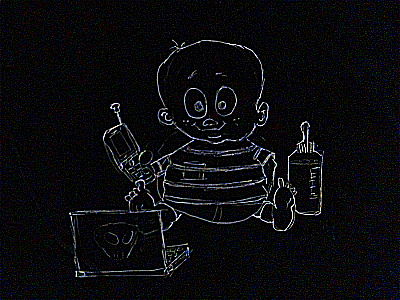
\includegraphics[width=2in]{org/art/getStartedHigh.png}\end{center}
\end{wrapfigure}

Nothing gives a better kick than working and releasing fast. The following code will get you a ``launching soon'' page ready with beta invite albeit manually. It requires node.js, an evented IO framework by Ryan Dahl. The code itself is written in coffeescript, a language by Jeremy Ashkenas.
First be comfortable with code and the fact that this small code will get us started and then we can move on to get it working.

\vspace{0.6cm}\lstinputlisting{app/stage1/server.coffee}\vspace{0.6cm}

%tip
\colorbox{tipcolour}{\tiny \textsc{Tip} \small Use commercial solutions like unbounce to set up quick sign up page}


\chapter{Working Model}
\begin{flushright}\textit{If it doesn't work, it doesn't exist.}\end{flushright}

\begin{wrapfigure}{r}{2in}
\begin{center}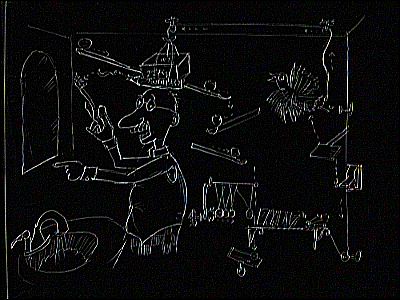
\includegraphics[width=2in]{org/art/workingModel.png}\end{center}
\end{wrapfigure}

Last stage was a baby's task. Lets get real and get a working model. To keep it simple, lets stick with simplest authentication via facebook and build upon existing hardwork. MongoDB will be used for storage, though a document based database is not really an ideal choice for the purpose. 

\end{document}
